\section{Exécution \& tests} % (fold)
\label{sec:execution}

A l'exécution l'utilisateur peut passer certains paramètres au programme. Ceux-ci sont les suivants :
\begin{itemize}
	\item $p$ : nombre de processus total. $p-1$ esclaves seront créés ;
	\item $t$ : nombre de threads de travail. Au total, $t+1$ threads sont créés, en comptant le thread de communication ;
	\item $r$ : longueur maximum des mots à vérifier ;
	\item $m$ : le mot de passe.
	\item $c$ : le chemin de l'exécutable \og slave\fg .
\end{itemize}

Il est ainsi possible de changer facilement les paramètres du programme entre deux exécutions, ce qui nous a permis de le tester pour un certain nombre de cas. \`A noter que le programme retourne une erreur si les paramètres ne sont pas cohérents (par exemple si $r$ est plus petit que la longueur du mot de passe).


\section{Performances} % (fold)
\label{sec:perf}

Pour les performances, nous avons créé un script qui nous permet de lancer des jobs sur la machine Plafrim de l'Inria. Le graphe de la figure \ref{fig:graph_procs} montre les résultats obtenus lorsque nous faisions varier le nombre de processus intervenant dans le calcul. Cependant, alors que nous voulions effectuer des tests supplémentaires afin de compléter nos observations, il s'est avéré que la machine Plafrim ne nous permettait plus de soumettre des jobs. 

\begin{figure}[h!]
\centering
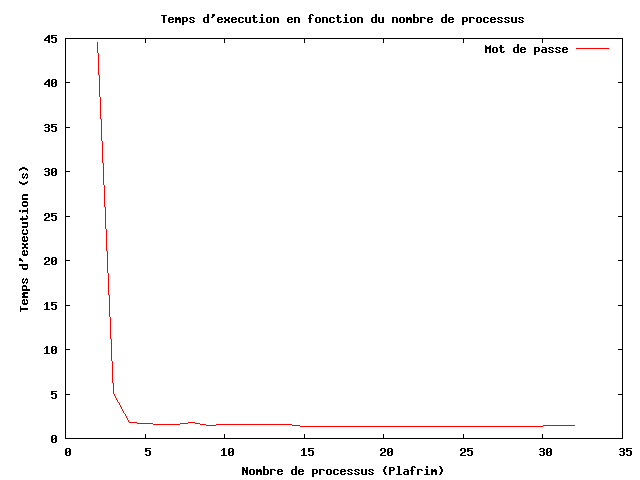
\includegraphics[width=0.8\textwidth]{1_graph_procs}
\caption{Résultats obtenus sur Plafrim}
\label{fig:graph_procs}
\end{figure}

